\chapter{KVM}
\label{chap:kvm}

KVM(Kernel-based Virtual Machin)的简称)是一个开源的系统虚拟化模块,
自Linux 2.6.20之后集成在Linux的各个主要发行版本中。它使用Linux自身的调
度器进行管理,所以相对于Xen,其核心源码很少。KVM目前已成为学术界的主
流VMM之一。

\section{关于KVM}
\label{sec:AboutKVM}

KVM是开源软件,全称是Kernel-based virtual machine(基于内核的虚拟机),
是x86架构且硬件支持虚拟化技术(如Intel VT-x或AMD-V)的Linux全虚拟化解决
方案。KVM包含一个为处理器提供底层虚拟化,可加载的核心模
块kvm.ko(kvm-intel.ko或kvm-amd.ko)。KVM还需要一个经过修改
的QEMU软件qemu-kvm,作为虚拟机上层控制和界面。

KVM能在不改变Linux或Windows镜像的情况下同时运行多个虚拟机(多个虚拟机使
用同一个镜像),并为每一个虚拟机配置个性化硬件环境(网卡、磁盘、图形适
配器等)。

在主流的Linux内核,如2.6.20以上的内核版本均已包含了KVM核心。

\subsection{KVM管理工具libvirt简介}
\label{sec:libvirtIntro}

libvirt是目前使用最为广泛的KVM虚拟机管理工具和应用程序接口(API),而且
一些常用虚拟机的管理工具(如virsh、virt-install及virt-manager等)和云计
算框架平台(如OpenStack、OpenNubla等)都在底层使用libvirt的应用程序接
口。

libvirt是为了更方便地管理平台虚拟化技术而设计的开放源代码的应用程序接口、
守护进程和管理工具,它不仅提供了对虚拟化客户机的管理,也提供了对虚拟化
网络和存储的管理。

libvirt的应用程序接口已被广泛地用在基于虚拟化和云计算的解决方案中,主要
作为连接底层Hypervisor和上层应用程序的一个中间适配层。libvirt对多种不同
的Hypervisor的支持是通过一种基于驱动程序的架构来实现的。libvirt对不同
的Hypervisor提供了不同的驱动:对Xen有Xen的驱动,对QEMU/KVM有QEMU驱动;
对VMware有VMware的驱动。libvirt作为中间适配层,让底层Hypervisor对上层用
户空间的管理工具是可以做到完全透明的,因为libvirt屏蔽了底层各
种Hypervisor的细节,为上层管理工具提供了一个统一的API接口。通过libvirt,
一些用户空间的管理工具可以管理各种不同的Hypervisor和其上面运行的客户机,
它们之间的交互拓扑如下图所示:

\begin{figure}[ht]
  \centering
  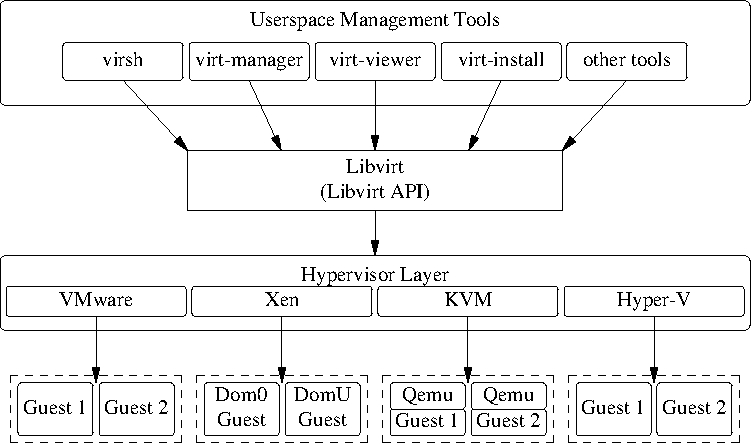
\includegraphics{graph/libvirt_support.pdf}
  \caption{\label{fig:libvirtSupport} Libvirt支持的虚拟化类型}
\end{figure}

\subsection{libvirt中的一些术语}
\label{sec:libvirtTerm}

1. 节点(Node):一台物理机;上面可能运行多个虚拟客户机,Hypervisor和Domain都运行在节点之上。

2. Hypervisor:也称虚拟机监视器(VMM),如KVM、Xen、VMware、Hyper-V等,是虚拟化中的一个底层软件层,它可以虚拟化一个节点让其运行多个虚拟客户机(不同的客户机有可能运行不同的操作系统)。

3. 域(Domain):是Hypervisor上运行的一个客户机操作系统实例。域也被称为实例、客户机操作系统(Guest OS)、虚拟机(Virtual Machine),它们都是指同一个概念。

节点、Hypervisor及域三者之间的关系如下图所示:

\begin{figure}[htbp]
  \centering
  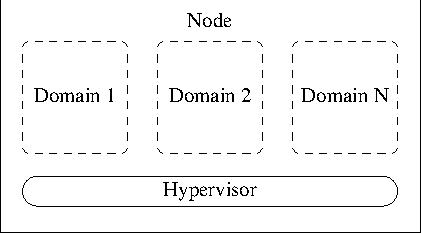
\includegraphics{graph/libvirt_node_hypervisor_domain.pdf}
  \caption{\label{fig:libvirtNodeHyperDomain} 节点、域与Hypervisor之间的关系}
\end{figure}

\subsection{检查宿主机是否支持KVM虚拟化}
\label{sec:checkIfSupportKVM}

\begin{verbatim}
# grep -E --color '(vmx|svm)' /proc/cpuinfo
\end{verbatim}

如果有红色的字符输出,说明系统支持虚拟化,然后接下来的一些操作才是有意
义的。

\section{安装前的准备工作}
\label{sec:kvmPrepare}

\subsection{KVM测试环境}
\label{sec:testEnv}

下面的操作是在VMWare的两台虚拟机上进行的,

测试环境为:

安装EPEL源

\subsection{安装EPEL源}
\label{sec:InstallEpel}

\begin{verbatim}
# rpm -ivh http://mirrors.ustc.edu.cn/fedora/epel//6/x86_64/epel-release-6-8.noarch.rpm
\end{verbatim}

\subsection{安装KVM管理工具}
\label{sec:InstallKvmManager}

为了使用KVM虚拟化,操作系统至少要安装qemu-kvm及qemu-img两个软件包,这两
个软件包在宿主机上为提使用者提供了用户层的KVM模拟器和硬盘镜像管理工具。
因此,这两个软件包是必须安装的,操作如下:

\begin{verbatim}
# yum install -y qemu-kvm qemu-img
\end{verbatim}

另外还有几个建议安装的软件包,如下:

安装以上建议的软件包:

\begin{verbatim}
# yum install virt-manager \
libvirt \
libvirt-python \
python-virtinst \
libvirt-client
\end{verbatim}

\section{开始部署KVM虚拟机}
\label{sec:beginKVM}

有了上面的准备工作,接下来就可以创建虚拟机了。

\subsection{创建虚拟机镜像}
\label{sec:createVmImg}

虚拟机镜像文件就是QEMU(KVM)虚拟机使用的硬盘文件格式。

\subsubsection{创建raw格式镜像文件}
\label{sec:createRawImg}

这里新建一个5G的RAW格式的虚拟镜像文件,可以根据具体业务设置镜像文件大小,

\begin{verbatim}
# qemu-img create -f raw /opt/lavenliu.raw 5G
Formatting '/opt/lavenliu.raw', fmt=raw size=5368709120
\end{verbatim}

创建完毕,可以查看刚才新建的虚拟机镜像文件,

\begin{verbatim}
# qemu-img info /opt/lavenliu.raw 
image: /opt/lavenliu.raw
file format: raw
virtual size: 5.0G (5368709120 bytes)
disk size: 0
\end{verbatim}

\subsubsection{创建qcow2格式镜像文件}
\label{sec:createQcow2Img}

创建qcow2格式的镜像文件与创建raw格式的镜像文件步骤一样,只是\verb|-f|选
项后面指定的虚拟机镜像文件格式不一样而已。操作如下:

\begin{verbatim}
# qemu-img create -f qcow2 /opt/taoqi.qcow2 5G
Formatting '/opt/taoqi.qcow2', fmt=qcow2 size=5368709120 encryption=off cluster_size=65536
\end{verbatim}

查看刚创建的虚拟机镜像文件,

\begin{verbatim}
# qemu-img info /opt/taoqi.qcow2 
image: /opt/taoqi.qcow2
file format: qcow2
virtual size: 5.0G (5368709120 bytes)
disk size: 1.4G
cluster_size: 65536
\end{verbatim}

format指镜像的格式,常用的格式为raw和qcow2,如果不声明,默认为raw模式,
但推荐使用qcow2格式。

\subsubsection{虚拟机镜像文件格式对比}
\label{sec:createImgContrast}

1.	raw格式:可以简单、容易地导出到其它模拟器中,但是立即分配占用空间大。
2.	qcow2格式:是qcow格式的升级版本,是目前最万能的格式。使用它可获得较小映像,也是虚拟池一直在使用的镜像格式,支持镜像快照,方便的恢复管理。

大量数据表明:qcow2格式的文件虽然在性能上比Raw格式的有一些损失(主要体
现在对于文件增量上,qcow2格式的文件为了分配cluster多花费了一些时间),
但是qcow2格式的镜像比Raw格式文件更小,只有在虚拟机实际占用了磁盘空间时,
其文件才会增长,能方便的减少迁移花费的流量,更适用于云计算系统,同时,
它还具有加密,压缩,以及快照等raw格式不具有的功能。

\subsection{安装虚拟机}
\label{sec:installVM}

接下来就进行虚拟机的安装,分别演示raw格式与qcow2格式的虚拟机镜像文件系统的安装。两者的系统安装基本上是一样的,不同的只是\verb|--disk|选项要指定不同的镜像文件格式而已。

\subsubsection{安装raw格式的虚拟机系统}
\label{sec:installRawVM}

有了上面的虚拟机镜像文件,相当于我们已经有了一个虚拟的硬盘了,接下来就
可以使用CentOS的ISO镜像文件,往这个新建的虚拟机镜像文件里安
装CentOS6u5的系统了。作者已事先准备好了CentOS6u5 64位的ISO系统镜像文件,
并存放在/opt/CentOS-6.5-x86\_64-bin-DVD1.iso。下面就演示如何进行安装,操
作如下:

\begin{verbatim}
# virt-install --virt-type kvm --name lavenliu --ram 512 \
   --cdrom=/opt/CentOS-6.5-x86_64-bin-DVD1.iso \
   --disk path=/opt/lavenliu.raw \
   --network network=default \
   --graphics vnc,listen=0.0.0.0 \
   --noautoconsole --os-type=linux \
   --os-variant=rhel6
\end{verbatim}

上述命令行参数的一些说明:

\subsubsection{安装qcow2格式的虚拟机系统}
\label{sec:installQcow2VM}

\begin{verbatim}
# virt-install --virt-type kvm --name taoqi --ram 512 \
   --cdrom=/opt/CentOS-6.5-x86_64-bin-DVD1.iso \
   --disk path=/opt/taoqi.qcow2,format=qcow2 \
   --network network=default \
   --graphics vnc,listen=0.0.0.0 \
   --noautoconsole --os-type=linux \
   --os-variant=rhel6
\end{verbatim}

上述命令行参数的一些说明:

安装过程中,libvirtd守护进程会监听5900和5901的两个VNC端口(因为启动了两
台虚拟机),供VNC客户端进行远程连接,可以查看kvm01服务器是否监
听5900及5901端口\footnote{如果同时安装N台虚拟机,则将分别监
  听5900、5901、\dots\ 、590N端口。},

\begin{verbatim}
# netstat -natup |grep 59
tcp    0      0 0.0.0.0:5900     0.0.0.0:*      LISTEN      20249/qemu-kvm      
tcp    0      0 0.0.0.0:5901     0.0.0.0:*      LISTEN      20268/qemu-kvm
\end{verbatim}

\section{KVM虚拟机管理}
\label{sec:manageKVM}

\subsection{libvirt的配置和使用}
\label{sec:configLibvirt}

libvirtd是一个作为libvirt虚拟化管理系统中的服务器端的守护进程,如果
要让某个节点能够用libvirt进行管理(无论是本地管理还是远程管理),都
需要在这个节点上运行着libvirtd这个守护进程,以便让其他上层管理工具
可以连接到该节点,libvirtd负责执行其他管理工具发送到它的虚拟化管理
操作指令。而libvirt的客户端工具(包括virsh、virt-manager等)可以连
接到本地货远程的libvirtd进程,以便管理节点上的客户机(启动、停止、
重启、迁移等)、收集节点上的宿主机和客户机的配置和资源使用状态。

默认情况下,libvirtd监听在本地的Unix Domain Socket上,并没有监听基
于网络的TCP/IP socket,需要使用"-l"或"--listen"的命令行参数来开启对
libvirtd.conf配置文件中对TCP/IP socket的配置。另外,libvirtd进程的
启动或停止,并不会直接影响正在运行的客户机。libvirtd在启动或重启完
成时,只要客户机的XML配置文件是存在的,libvirtd会自动加载这些客户机
的配置文件,获取它们的信息;当然,如果客户机没有基于libvirt格式的
XML文件来运行,libvirtd则不能发现它。

\subsection{虚拟机拷贝}
\label{sec:copyVM}

虚拟机的拷贝,其实可以理解为复制某一台虚拟机的XML文件为一个新的XML配置
文件,然后重新define这个新的XML文件即可。不过为了能够让新的虚拟机正常工
作,需要修改新的XML文件的几处配置,大致的步骤为:

dump某台虚拟机的XML配置文件到新的XML配置文件

复制某台虚拟机的镜像文件到新的镜像文件

修改新的XML配置文件的相应配置

修改新的虚拟机的MAC地址

操作如下:

\begin{verbatim}
# virsh dumpxml lavenliu > lavenliu_new.xml
# cp /opt/lavenliu.raw /opt/lavenliu_new.raw
# sed -i 's#lavenliu#lavenliu_new#g' /opt/lavenliu_new.xml
# sed -i "s#<uuid>.*</uuid>#<uuid>`uuidgen`</uuid>#g" /opt/lavenliu_new.xml
# sed -i "s@<mac address=.*@<mac address='`printf '00:0C:%02X:%02X:%02X:%02X\n' $((RANDOM%256)) $((RANDOM%256)) $((RANDOM%256)) $((RANDOM%256))`'/>@g" /opt/taoqi-new.xml
\end{verbatim}

注意,还要修改MAC地址,不然两台虚拟机的MAC地址是一样的。

使用这种复制虚拟机镜像文件的方式,需要修改修改虚拟机的xml配置文件。验证上述步骤是否成功,操作如下:

\begin{verbatim}
# virsh list --all
 Id    Name                           		State
----------------------------------------------------
 16    lavenliu                       	running
 -     lavenliu_new                   	shut off  # 已经创建成功,但未启动
 -     taoqi                          		shut off
\end{verbatim}

接下来启动lavenliu\_new虚拟机,是否可以启动,

\begin{verbatim}
# virsh list 
 Id    Name                           		State
----------------------------------------------------
 16    lavenliu                       	running
 17    lavenliu_new                   	running
\end{verbatim}

\subsection{虚拟机克隆}
\label{sec:cloneVM}

克隆虚拟机时,虚拟机必须要处于关闭或暂停状态。否则,将会出现下面的提示:

\begin{verbatim}
ERROR    Domain with devices to clone must be paused or shutoff.
\end{verbatim}

克隆虚拟机操作如下:

\begin{verbatim}
# virt-clone -o lavenliu -n lavenliu_clone -f /opt/lavenliu_clone.raw
Cloning lavenliu.raw       | 5.0 GB     02:33     

Clone 'lavenliu_clone' created successfully.
\end{verbatim}

相应选项说明:

\begin{verbatim}
-o 指定源虚拟机
-n 指定新虚拟机
-f 指定新虚拟机的镜像文件
\end{verbatim}

查看已克隆的虚拟机:

\begin{verbatim}
# ll /opt/
total 8217244
-rwxr-xr-x  1 root root 5368709120 Apr 26 18:11 lavenliu_clone.raw
-rw-r--r--  1 root root 5368709120 Apr 26 18:08 lavenliu.raw
drwxr-xr-x. 2 root root       4096 Nov 22  2013 rh
-rw-r--r--  1 root root 1517944832 Apr 26 17:16 taoqi.qcow2
\end{verbatim}

能否启动呢?试试看:

\begin{verbatim}
# virsh list --all
 Id    Name                          State
----------------------------------------------------
 18    lavenliu_new            running
 -        lavenliu                     shut off
 -        lavenliu_clone          shut off
 -        taoqi                          shut off
\end{verbatim}

接下来启动刚克隆的lavenliu\_clone虚拟机,

\begin{verbatim}
# virsh start lavenliu_clone
Domain lavenliu_clone started
\end{verbatim}

查看运行状态:

\begin{verbatim}
# virsh list --all
 Id     Name                       State
----------------------------------------------------
 18    lavenliu_new          running
 19    lavenliu_clone        running  # 启动成功
 -        lavenliu                   shut off
 -        taoqi                        shut off
\end{verbatim}



\subsection{增加虚拟机硬盘空间}
\label{sec:scaleVmDisk}

对硬盘做操作要谨慎。要做好备份再进行操作比较可靠。

\begin{verbatim}
# cd /opt
# qemu-img info lavenliu.raw 
image: lavenliu.raw
file format: raw
virtual size: 5.0G (5368709120 bytes)
disk size: 1.4G
# qemu-img resize lavenliu.raw +1G
Image resized.
# qemu-img info lavenliu.raw 
image: lavenliu.raw
file format: raw
virtual size: 6.0G (6442450944 bytes)
disk size: 1.4G
\end{verbatim}

\subsection{虚拟机硬盘格式转换}
\label{sec:convertVmDisk}

把raw格式的硬盘转换为qcow2格式的,

\begin{verbatim}
# cd /opt
# qemu-img convert -c -f raw -O qcow2 lavenliu.raw new.qcow2
# 格式转换需要一段时间
# qemu-img check new.qcow2
No errors were found on the image.
Image end offset: 491454464
\end{verbatim}

上述命令选项说明:

\begin{verbatim}
-c 表示压缩,对qcow2格式的镜像文件
-f 要被转换的格式
-O 转换后的格式
lavenliu.raw # 要被转换的镜像文件
new.qcow2 # 转换后的镜像文件
\end{verbatim}

然后直接使用vim修改lavenliu.xml文件后,reboot虚拟机后,其磁盘格式仍然是raw格式。彻底更改使用"virsh edit new"。在生产环境中使用virsh edit xxx来修改设置。

\subsection{虚拟机迁移}
\label{sec:moveVM}

尽量避免使用动态迁移。可以使用复制的静态方式来迁移虚拟机,然后重新定义虚拟机的XML文件。

\subsection{创建虚拟机快照}
\label{sec:createSnapShot}

要创建虚拟机快照,首先要满足以下几个条件:

虚拟机使用的镜像文件格式为qcow2格式;

进行快照操作时,虚拟机最好处于关闭或暂停的状态;

关于快照相关的命令语法为:

\begin{verbatim}
# qemu-img snapshot [-l | -a snapshot | -c snapshot | -d snapshot] filename
\end{verbatim}

命令行参数说明:

\begin{verbatim}
qemu-img snapshot 
-l # 查看虚拟机快照
-a snapshot # 应用指定的快照
-c snapshot # 创建快照
-d snapshot # 删除指定的快照
\end{verbatim}

\subsubsection{创建虚拟机快照}
\label{sec:createVmSnapShot}

先来个错误的操作,对raw格式的虚拟机镜像文件创建快照,

\begin{verbatim}
# qemu-img snapshot -c 1st_snapshot /opt/lavenliu.raw 
Could not create snapshot '1st_snapshot': -95 (Operation not supported)
\end{verbatim}

结果给出了错误提示:“Operation not supported”。

接下来对taoqi这台虚拟机先进行关闭操作,然后再进行创建快照操作(最好关闭或暂停虚拟机),

\begin{verbatim}
# virsh destroy taoqi
# qemu-img snapshot -c 1st_snapshot /opt/taoqi.qcow2
\end{verbatim}

如果没有提示,说明创建成功。在UNIX世界中,没有消息就是好消息。接下来我们可以登录到taoqi这台虚拟机里,创建一个测试文件,如在/root目录下创建一个名为taoqi.iso的文件,操作如下:

\begin{verbatim}
# dd if=/dev/zero of=/root/taoqi.iso bs=1M count=256
\end{verbatim}

这时可以再次对taoqi这台虚拟机创建第2个快照,操作如下:

\begin{verbatim}
# qemu-img snapshot -c 2nd_snapshot /opt/taoqi.qcow2
\end{verbatim}

\subsubsection{查看虚拟机快照}
\label{sec:listVmSnapShot}

以上我们都创建了两个快照了,怎么查看呢?以及创建的快照文件存放在何处呢?接下来看操作:

\begin{verbatim}
# qemu-img snapshot -l /opt/taoqi.qcow2 
Snapshot list:
ID        TAG                 VM SIZE                DATE       VM CLOCK
1         1st_snapshot             0 2016-04-26 20:48:58   00:00:00.000
2         2nd_snapshot           0 2016-04-26 20:49:52   00:00:00.000
\end{verbatim}

\subsubsection{恢复指定快照}
\label{sec:resumeSpecificVmSnapShost}

这时我们恢复到第一个快照,我们在做完第一个快照后,创建了一个/root/test.iso的文件,那么当我们恢复到第一个快照时,在/root目录下应该是没有test.iso文件的,是不是这样的呢?接下来看操作:

\begin{verbatim}
# virsh destroy taoqi
# qemu-img snapshot -a 1st_snapshot /opt/taoqi.qcow2
# virsh start taoqi
\end{verbatim}

登录到taoqi这台虚拟机进行查看,发现/root/test.iso文件没有了(肯定没有改文件,因为在创建1st\_snapshot时,还没有创建/root/test.iso文件的,所以恢复到1st\_snaphost快照时是看不到创建快照后的文件)。

恢复2nd\_snapshot快照,

\begin{verbatim}
# virsh destroy taoqi
# qemu-img snapshot -a 2nd_snapshot /opt/taoqi.qcow2
# virsh start taoqi
\end{verbatim}

登录到taoqi这台虚拟机,查看/root目录,test.iso文件是不是又回来了。

\subsubsection{删除虚拟机快照}
\label{sec:deleteVmSnapShot}

删除快照很简单,把相应的选项换成\verb|-d|就可以了,首先查看当前有哪些快照,操作如下:

\begin{verbatim}
# qemu-img snapshot -l /opt/taoqi.qcow2 
Snapshot list:
ID        TAG                 VM SIZE                DATE       VM CLOCK
1         1st_snapshot              0 2016-04-27 12:08:24   00:00:00.000
2         2nd_snapshot              0 2016-04-27 12:45:27   00:00:00.000
\end{verbatim}

接下来删除第一个快照,

\begin{verbatim}
# qemu-img snapshot -d 1st_snapshot /opt/taoqi.qcow2
\end{verbatim}

\section{KVM虚拟机桥接网络}
\label{sec:kvmBridgeNetwork}

默认情况下,虚拟机的网络使用的是NAT的方式。使用ifconfig命令查看宿主机的网络接口情况:

\begin{verbatim}
# ifconfig 
eth0     Link encap:Ethernet  HWaddr 00:0C:29:1C:1F:8E  
          inet addr:192.168.19.134  Bcast:192.168.19.255  Mask:255.255.255.0
          inet6 addr: fe80::20c:29ff:fe1c:1f8e/64 Scope:Link
          UP BROADCAST RUNNING MULTICAST  MTU:1500  Metric:1
          RX packets:25557 errors:0 dropped:0 overruns:0 frame:0
          TX packets:14455 errors:0 dropped:0 overruns:0 carrier:0
          collisions:0 txqueuelen:1000 
          RX bytes:25142063 (23.9 MiB)  TX bytes:834829 (815.2 KiB)

eth1     Link encap:Ethernet  HWaddr 00:0C:29:1C:1F:98  
          inet addr:192.168.20.129  Bcast:192.168.20.255  Mask:255.255.255.0
          inet6 addr: fe80::20c:29ff:fe1c:1f98/64 Scope:Link
          UP BROADCAST RUNNING MULTICAST  MTU:1500  Metric:1
          RX packets:41832 errors:0 dropped:0 overruns:0 frame:0
          TX packets:39199 errors:0 dropped:0 overruns:0 carrier:0
          collisions:0 txqueuelen:1000 
          RX bytes:3197973 (3.0 MiB)  TX bytes:13961170 (13.3 MiB)

lo        Link encap:Local Loopback  
          inet addr:127.0.0.1  Mask:255.0.0.0
          inet6 addr: ::1/128 Scope:Host
          UP LOOPBACK RUNNING  MTU:16436  Metric:1
          RX packets:13 errors:0 dropped:0 overruns:0 frame:0
          TX packets:13 errors:0 dropped:0 overruns:0 carrier:0
          collisions:0 txqueuelen:0 
          RX bytes:2828 (2.7 KiB)  TX bytes:2828 (2.7 KiB)

virbr0   Link encap:Ethernet  HWaddr 52:54:00:F0:29:34  
          inet addr:192.168.122.1  Bcast:192.168.122.255  Mask:255.255.255.0
          UP BROADCAST RUNNING MULTICAST  MTU:1500  Metric:1
          RX packets:431 errors:0 dropped:0 overruns:0 frame:0
          TX packets:341 errors:0 dropped:0 overruns:0 carrier:0
          collisions:0 txqueuelen:0 
          RX bytes:41451 (40.4 KiB)  TX bytes:42172 (41.1 KiB)

vnet0    Link encap:Ethernet  HWaddr FE:54:00:CC:94:60  # lavenliu这台虚拟机的MAC地址
          inet6 addr: fe80::fc54:ff:fecc:9460/64 Scope:Link
          UP BROADCAST RUNNING MULTICAST  MTU:1500  Metric:1
          RX packets:12 errors:0 dropped:0 overruns:0 frame:0
          TX packets:156 errors:0 dropped:0 overruns:0 carrier:0
          collisions:0 txqueuelen:500 
          RX bytes:1112 (1.0 KiB)  TX bytes:8548 (8.3 KiB)

vnet1    Link encap:Ethernet  HWaddr FE:54:00:18:DF:60  # taoqi这台虚拟机的MAC地址
          inet6 addr: fe80::fc54:ff:fe18:df60/64 Scope:Link
          UP BROADCAST RUNNING MULTICAST  MTU:1500  Metric:1
          RX packets:27 errors:0 dropped:0 overruns:0 frame:0
          TX packets:1174 errors:0 dropped:0 overruns:0 carrier:0
          collisions:0 txqueuelen:500 
          RX bytes:2636 (2.5 KiB)  TX bytes:63308 (61.8 KiB)
\end{verbatim}

查看系统的ARP缓存列表:

\begin{verbatim}
# arp
Address			HWtype  HWaddress			Flags Mask	Iface
192.168.20.1		ether   00:50:56:c0:00:01	C 				eth1
192.168.122.141	ether   52:54:00:cc:94:60	C				virbr0
192.168.19.2		ether   00:50:56:ea:9c:68	C				eth0
192.168.122.41	ether   52:54:00:18:df:60	C				virbr0
\end{verbatim}

使用brctl命令查看:

\begin{verbatim}
# brctl show
bridge name	bridge id				STP enabled	interfaces
virbr0			8000.525400f02934	yes			virbr0-nic
														vnet0
														vnet1
\end{verbatim}

当我们要在局域网中访问宿主机上的虚拟机时,这时使用桥接网络将显得很有必要。接下来在kvm02.lavenlilu.com主机上创建kvm-bridge虚拟机并使用桥接的方式,可以让局域网中的其他机器可以访问到它(如从kvm01.lavenliu.com主机可以访问kvm02上的kvm-bridge虚拟机)。操作如下,然后在宿主机上增加网桥设备br1,

\begin{verbatim}
# virsh iface-bridge eth1 br1
Created bridge br1 with attached device eth1
Bridge interface br1 started
\end{verbatim}

上面的命令执行完毕,将会在/etc/sysconfig/network-scripts/目录中产生ifcfg-br1网络接口文件,内容如下:

\begin{verbatim}
# cat /etc/sysconfig/network-scripts/ifcfg-br1
DEVICE="br1"
ONBOOT="yes"
TYPE="Bridge"
BOOTPROTO="none"
IPADDR="192.168.20.130"
NETMASK="255.255.255.0"
GATEWAY="192.168.20.1"
STP="on"
DELAY="0"
\end{verbatim}

网卡接口文件ifcfg-eth1上的信息也会被virsh工具修改,IP地址被删除了,内容如下:

\begin{verbatim}
# cat /etc/sysconfig/network-scripts/ifcfg-eth1
DEVICE=eth1
ONBOOT=yes
BRIDGE="br1"
\end{verbatim}

使用brctl show命令查看当前桥接情况:

\begin{verbatim}
# brctl show
bridge name	bridge id		STP enabled	interfaces
br1		8000.000c2948b730	yes		eth1
\end{verbatim}

接下来创建新的kvm-bridge虚拟机镜像文件,并安装系统:

\begin{verbatim}
# qemu-img create -f qcow2 /opt/kvm-bridge.qcow2
# virt-install --virt-type kvm --name kvm-bridge \
--ram 512 \
--cdrom=/opt/CentOS-6.5-x86_64-bin-DVD1.iso \
--disk path=/opt/kvm-bridge.qcow2,format=qcow2 \
--network bridge=br1 \
--graphics vnc,listen=0.0.0.0 \
--noautoconsole \
--os-type=linux \
--os-variant=rhel6

Starting install...
Creating domain...                      |    0 B     00:01     
Domain installation still in progress. You can reconnect to 
the console to complete the installation process.
\end{verbatim}

等待虚拟机操作系统安装完毕,可以查看当前宿主机的网络桥接情况,

\begin{verbatim}
# brctl show
bridge name	bridge id			                STP enabled		interfaces
br1			8000.000c2948b730		  yes		              eth1
														              vnet0
\end{verbatim}

可以在我们的Windows机器上进行ping测试,是否可以连通我们的kvm-bridge虚拟机(这里的虚拟机IP地址为192.168.20.117),

\begin{verbatim}
ping 192.168.20.117

正在 Ping 192.168.20.117 具有 32 字节的数据:
来自 192.168.20.117 的回复: 字节=32 时间<1ms TTL=64
来自 192.168.20.117 的回复: 字节=32 时间<1ms TTL=64
来自 192.168.20.117 的回复: 字节=32 时间<1ms TTL=64
来自 192.168.20.117 的回复: 字节=32 时间<1ms TTL=64

192.168.20.117 的 Ping 统计信息:
    数据包: 已发送 = 4,已接收 = 4,丢失 = 0 (0% 丢失),
往返行程的估计时间(以毫秒为单位):
    最短 = 0ms,最长 = 0ms,平均 = 0ms
\end{verbatim}

至此,虚拟机使用桥接网络可以被局域网中的其他机器访问。

\section{Libvirt API}
\label{sec:libvirtAPI}

\subsection{Libvirt API简介}
\label{sec:introLibvirtAPI}

libvirt的核心价值和主要目标就是提供了一套管理虚拟机的、稳定的、高效的应
用程序接口(API)。libvirt API本身是用C语言实现的,

\subsection{C API示例}
\label{sec:libvirtCAPI}

在使用libvirt API之前,必须要在远程或本地节点上启动libvirtd守护进程。在
使用libvirt的客户端,需要安装libvirt-devel开发包,如果没有安装,请执行如下操作进行安装:

\begin{verbatim}
# yum install -y libvirt-devel
\end{verbatim}

编写源代码时,需要在源码的开头引入\verb|<libvirt/libvirt.h>|头文件,编写完毕源
代码,如何编译呢?

\begin{verbatim}
# gcc test.c -o test -lvirt
\end{verbatim}

\subsubsection{显示某个域的信息}
\label{sec:displayDomainInfo}

代码如下:

\begin{verbatim}
# cat dominfo.c 
/**
 * Get domain information via libvirt C API.
 * Tested with libvirt-devel- on CentOS6.5 host system
 */

#include <stdio.h>
#include <libvirt/libvirt.h>

int getDomainInfo(int id)
{
    virConnectPtr conn = NULL; /* the hypervisior connection */
    virDomainPtr dom = NULL; /* the domain being checked */
    virDomainInfo info; /* the information being fetched */

    /* NULL means connect to local QEMU/KVM hypervisor*/
    conn = virConnectOpenReadOnly(NULL);
    if (conn == NULL) {
      fprintf(stderr, "Failed to connect to hypervisor\n");
      return 1;
    }

    /* find the Domain by its ID*/
    dom = virDomainLookupByID(conn, id);
    if (dom == NULL) {
      fprintf(stderr, "Failed to find Domain %d\n", id);
      virConnectClose(conn);
      return 1;
    }

    /* Get virDomainInfo structure of the domain */
    if (virDomainGetInfo(dom, &info) < 0) {
      fprintf(stderr, "Failed to get information for Domain %d\n", id);
      virDomainFree(dom);
      virConnectClose(conn);
      return 1;
    }

    /* Print some info of the domain*/
    printf("Domain ID: %d\n", id);
    printf("  vCPUs: %d\n", info.nrVirtCpu);
    printf("  maxMem: %d KB\n", info.maxMem);
    printf("  memory: %d KB\n", info.memory);

    if (dom != NULL)
      virDomainFree(dom);
    if (conn != NULL)
      virConnectClose(conn);

    return 0;
}

int main(int argc, char *argv[])
{

    int dom_id = 5;
    printf("-- Get Domain info by ID via libvirt C API --\n");
    getDomainInfo(dom_id);
    return 0;
}
\end{verbatim}

编译并运行:

\begin{verbatim}
# gcc dominfo.c -o dominfo -lvirt
./dominfo
-- Get Domain info by ID via libvirt C API --
Domain ID: 5
  vCPUs: 1
  maxMem: 524288 KB
  memory: 524288 KB
\end{verbatim}


\subsection{Python API示例}
\label{sec:libvirtPythonAPI}

许多种语言都提供了libvirt的绑定。Python作为一种在Linux上比较流行的编程语言,它也提供了libvirt API的绑定。在使用Python调用libvirt API之前,需要安装libvirt-python软件包,如果没有安装则执行如下命令进行安装:

\begin{verbatim}
# yum install -y libvirt-python
\end{verbatim}

\subsubsection{查看宿主机正在运行的虚拟机}
\label{sec:displayDomainInfo}

\begin{verbatim}
#!/usr/bin/env python
# coding: utf-8

# Get domain info via libvirt python API
# Tested with python2.6 and libvirt-python-0.10.2 on KVM host.

import libvirt
import sys


def createConnection():
    conn = libvirt.openReadOnly(None)
    if conn is None:
        print 'Failed to open connection to QEMU/KVM'
        sys.exit(1)
    else:
        print '-- Connection is created successfully --'
    return conn


def closeConnection(conn):
    """
    Arguments:
    - `conn`:
    """
    print
    try:
        conn.close()
    except:
        print 'Failed to close the connection'
        return 1
    print 'Connection is closed'


def getDomInfoByName(conn, name):
    """
    Arguments:
    - `conn`:
    - `NameError`:
    """
    print
    print '---- get domain info by name ----'
    
    try:
        myDom = conn.lookupByName(name)
    except:
        print 'Failed to find the domain with name "%s"' % name
        return 1
    
    print "Dom id: %d name: %s" % (myDom.ID(), myDom.name())
    print "Dom state: %s" % myDom.state(0)
    print "Dom info: %s" % myDom.info()
    print "memory: %d MB" % (myDom.maxMemory() / 1024)
    print "memory status: %s" % myDom.memoryStats()
    print "vCPUs: %d" % myDom.maxVcpus()


def getDomInfoByID(conn, id):
    """
    Arguments:
    - `conn`:
    - `id`:
    """
    print
    print '---- get domain info by ID ----'
    try:
        myDom = conn.lookupByID(id)
    except:
        print 'Failed to find the domain with ID "%d"' % id
        return 1
    print "Domain id is %d; Name is %s" % (myDom.ID(), myDom.name())


if __name__ == '__main__':
    name1 = "kvm-demo"
    name2 = "new"
    id1 = 5
    id2 = 6
    print '-- Get domain info via libvirt python API --'
    conn = createConnection()
    getDomInfoByName(conn, name1)
    getDomInfoByName(conn, name2)
    getDomInfoByID(conn, id1)
    getDomInfoByID(conn, id2)
    closeConnection(conn)
\end{verbatim}

%%% Local Variables:
%%% mode: latex
%%% TeX-master: t
%%% End:
